\ifx\frameselection\somethingundefined
\def\frameselection{1-4}
\fi

\def\pasteframeselection#1{\begin{frame}<#1>}%
\expandafter\pasteframeselection\expandafter{\frameselection}%
[label=codeoverview]
\frametitle{Code vs \lang,Visual,Visueel,}

\parbox[c][0.8\textheight]{0.35\textwidth}{
    \begin{itemize}
        \item<1-> Websites \& Apps
        \par\uncover<3->{
            \textbf{Complex}
        }
        
        \item<4-> Wikipedia
        \par\uncover<5->{
            \textbf{Consistent}
        }

        \item<6-> WhatsApp
        \par\uncover<7->{
            \textbf{\lang,Expandable,Uitbreidbaar,}
        }
    \end{itemize}
}\hfil
%\parbox[c]{1pt}{\textcolor{red}{\rule{0.5pt}{0.3\textheight}}}%
\hfil
\parbox[c]{0.6\textwidth}{
    \unless\ifishandout
    \only<1>{
        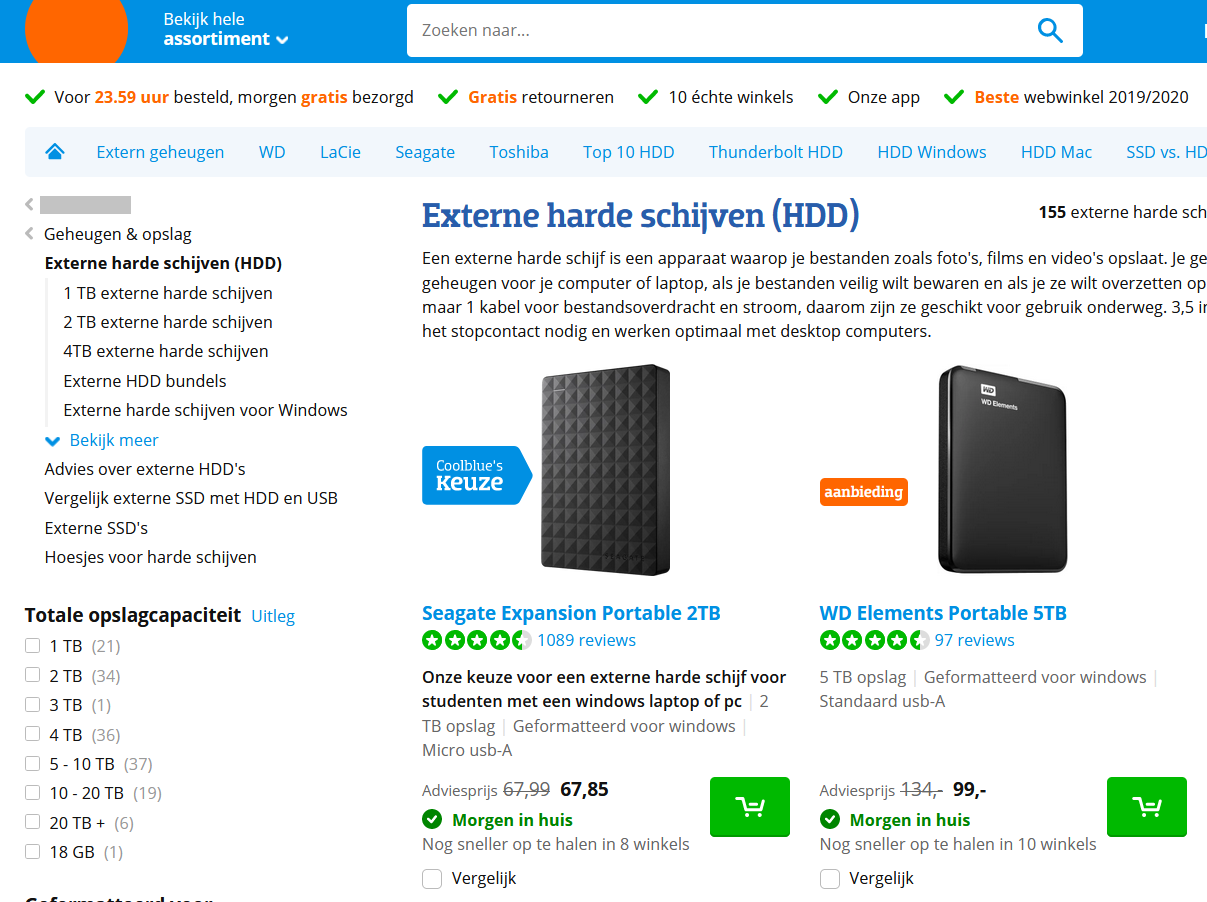
\includegraphics[
            width=\linewidth,height=0.8\textheight,keepaspectratio
        ]{assets/websiteVisual.png}
    }
    \only<2-3>{
        \adjustbox{
            trim=0pt {0.5\height} {0.5\width} 0pt,clip,width=\linewidth
        }{%
            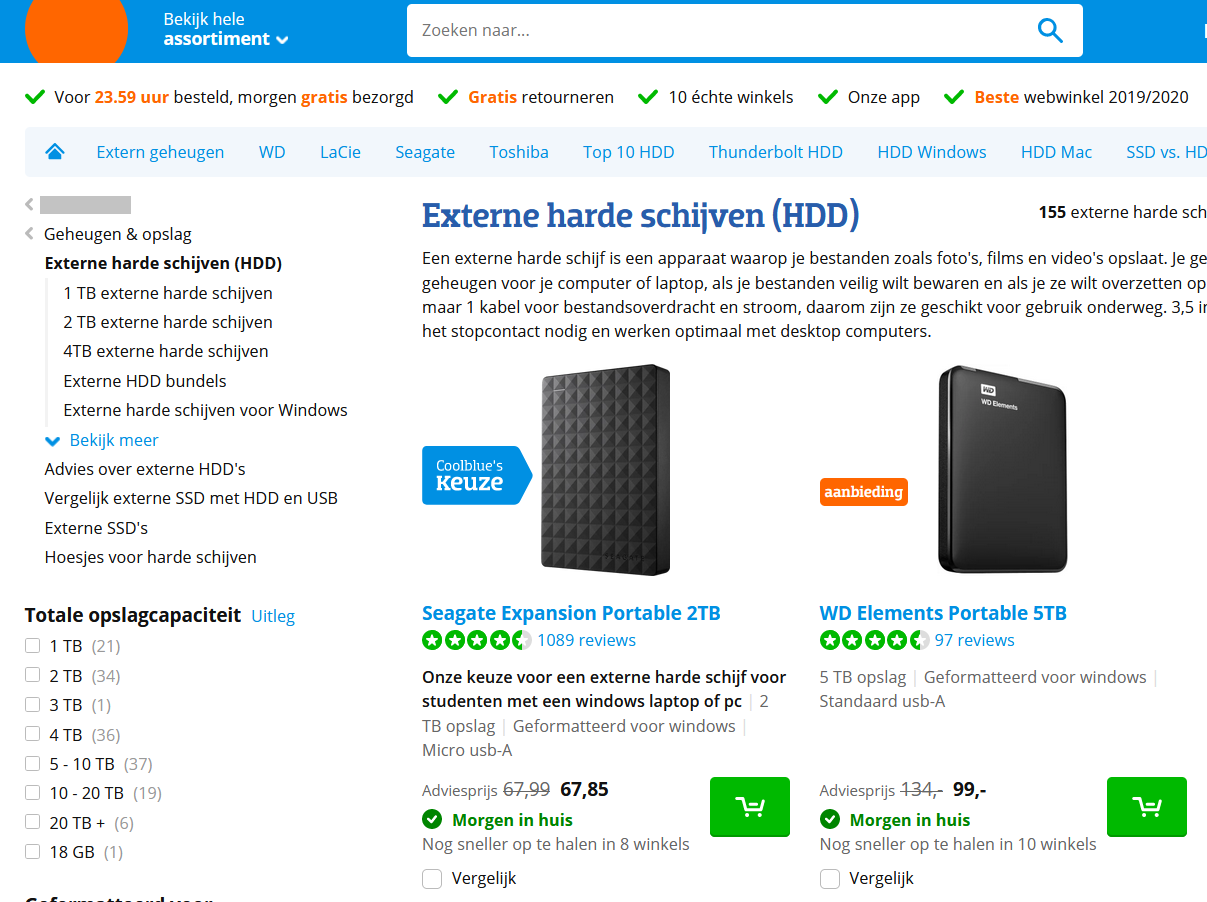
\includegraphics[
                width=\linewidth,height=0.8\textheight,keepaspectratio
            ]{assets/websiteVisual.png}%
        }
    }
    \only<4-5>{
        \centering
        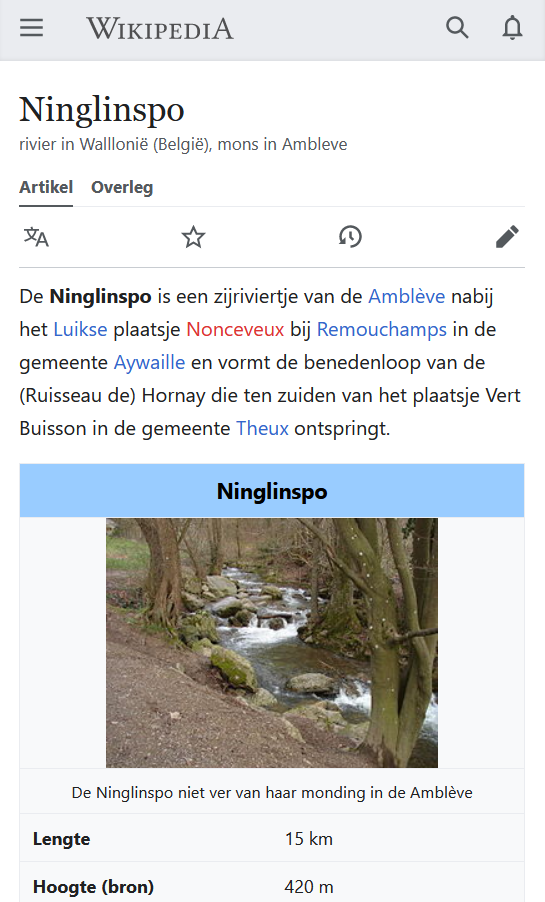
\includegraphics[width=\linewidth,height=0.8\textheight,keepaspectratio]{assets/wikipediaVisual}
        %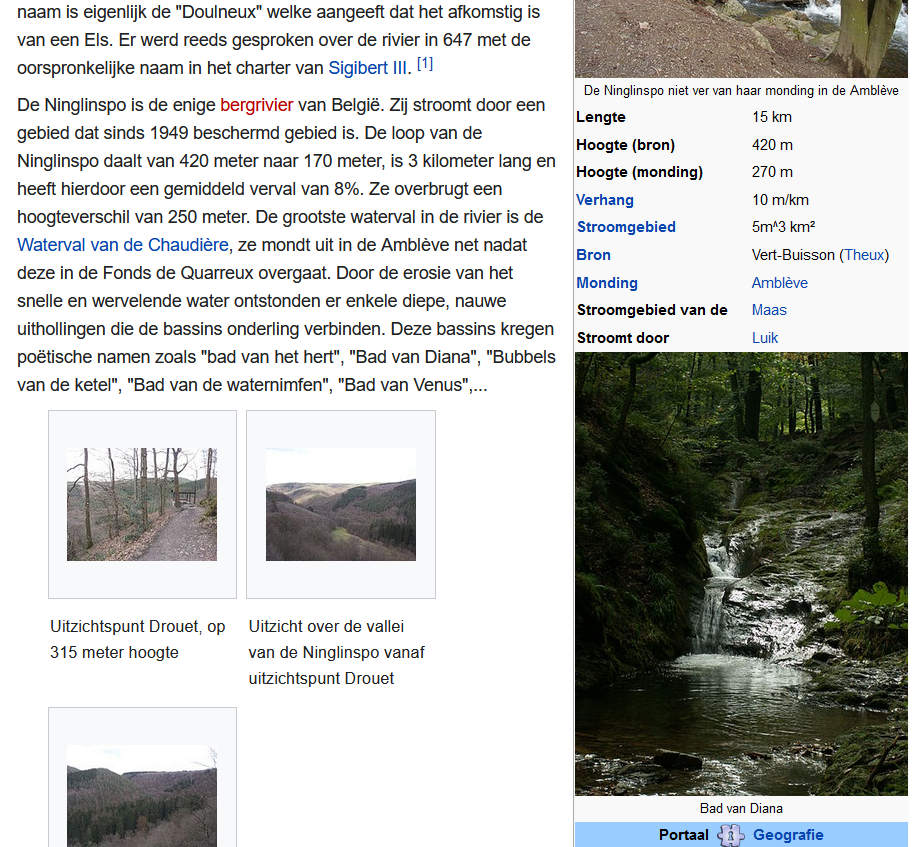
\includegraphics[width=\linewidth,height=0.8\textheight,keepaspectratio]{assets/wikipediaVisual2}
    }
    \fi
    \only<6-7>{
        
\includegraphics[width=\linewidth]{assets/whatsappStyles2.png}
        
        \bigskip
        
        %
\includegraphics[width=\linewidth]{whatsappStylesResultCropped.jpg}
        
\includegraphics[width=\linewidth]{assets/whatsappStylesResult2.png}
    }
}
\end{frame}

\let\frameselection\somethingundefined
